%\subsection{Updated Byrd ice core chronology}\label{agedepthresults}
%\textbf{The 5,000-year accumulation function gives the best fit of the volcanic observations at the Byrd ice core, so it is used in the final ice flow model effort. The resulting uncertainties in radar depth and age to each of the layers of interest in shown in Table~\ref{tab:depthunc}. For the deepest observed reflector that can be traced between WAIS Divide ice core and Byrd ice core, the depth and age uncertainty are 0.3\% and 5\%, respectively, at the 1$\sigma$ level. The mean and median ages and depths are consistent due to the gaussian nature of the errors, as shown in Figure~\ref{fig:layer_agedepth}.}

\subsection{Reflector age and parameter estimates}
The marginal probability distributions (1-D projections of the joint probability) of age and depth derived for englacial radar reflectors observed at the Byrd ice core site are shown in Figure~\ref{fig:layer_histo} and Table~\ref{tab:depthunc}. The age of the observed reflectors increases with depth, as expected due to stratigraphic burial of ice as it is deposited at the ice sheet surface. However, uncertainty in depth (and therefore age) does not increase monotonically with depth because of its dependence on reflector signal to noise ratio (SNR), as discussed in the next section. %and span to before the Last Glacial Maximum with 
We estimate the oldest continuous radar reflector in central West Antarctica to be 24.9 $\pm$ 0.3 ka despite being observed at only 68\% of the ice column depth (1466 $\pm$ 5 m). While this constrains the age of ice near the bed of the ice sheet, it also limits the ability to use radar observations in this area to directly study ice sheet dynamics before the Last Glacial Maximum. Reflector 3, the second deepest reflector, is dated to 17.2 $\pm$ 0.4 ka which is consistent with the estimated age of the ``Old Faithful" reflector, believed to be a relict from a series of volcanic eruptions. Reflectors 1 and 2 sample the ice column during the last 10 ka.%, with Reflector 1 dated to 4.72 $\pm$ 0.2 ka, around the time of an abrupt rise in dust flux at the end of the African Humid Period \citep{tierney2013,mcgee2013,shanahan2015}.

As has been established in previous work \citep{siegert1998,dowdeswell2004}, we assume radar reflectors are isochronous such that their age is the same whether observed at the Byrd ice core or the WAIS Divide ice core. To compare between the two ice cores, we use Halliburton's Landmark seismic interpretation software to track radar reflectors through central WAIS via an existing radar survey flight line (Figure~\ref{fig:radarmap}). The age-depth profiles at the Byrd ice core site (this study) and the WAIS Divide ice core effort \citep{buizert2015} are shown in Figure~\ref{fig:spaghetti}. Mean estimated age for each reflector at the Byrd ice core site compares favorably to that computed at the WAIS Divide ice core site (Figure~\ref{fig:spaghetti}).  

In addition to computing the age and depth of radar reflectors, our method includes inversion for a number of parameters related to ice flow and paleo accumulation rates (Table~\ref{tab:paramvals}) . Posterior probability distributions for these parameters are shown in Figure~\ref{fig:paramhist}. Estimates of accumulation rate are uncertain, particularly in the brittle zone of the Byrd ice core (300 m to 900 m) where volcanic data are not available and corresponding posterior distributions look most non-gaussian. The widest, most uncertain accumulation rate posterior distribution represents depths below the deepest volcanic records ($\sim$1850 m), where there is limited constraints on the estimate. Even with these limitations, the general pattern of estimated accumulation rate reflects an expected pattern of lower accumulation rate during the Last Glacial Maximum ($\sim$1500 m), where we infer accumulation rates about half that of the modern (Figure~\ref{fig:accumdepth}). 

Posterior probability distributions for other ice flow parameters estimated by the model are also shown in Figure~\ref{fig:paramhist}. The ratio of surface to bed velocity, $q$, is inferred to be 0.9 $\pm$ 0.08 (where a ratio of 1 would indicate plug flow) indicating near plug flow at the Byrd ice core, which is consistent with the presence of liquid water at the ice sheet base found during drilling. The transition depth, $h$, is not well constrained by our estimates, likely because of the near-plug-flow conditions inferred by our model.
%is estimated to be in the bottom 23\% of the ice column, between 1335 and 1989 m depth, which roughly corresponds to the where the deepest reflector is observed, below which is an echo-free zone. 
%suggesting additional deformation in the bottom 25\% of the ice column. %We find the firn correction, $d_{firn}$, has relatively large uncertainty (30 $\pm$ 8.4 m) and 
We estimate the mean radar velocity through ice, $v_{ice}$, to be 168.4 $m/{\mu}s$ which is in the middle the range suggested by empirical estimates, but our posterior probablity distribution shows secondary peaks. Estimates of the precision parameter $S$ imply 2.5\% uncertainty in reflector age with a 95\% confidence interval of [1.8\%, 4.11\%] (from $S \sim \frac{1}{\sigma^2}$)%. This is also combined with the nominally-assumed 1\% uncertainty introduced in $\sigma_{A}$ and suggests several percent uncertainty in the reflector chronology
, consistent with values that have been reported in ice core chronologies.

%Finally, estimates of the depth to the four radar reflectors used in this study show consistent uncertainty regardless of depth, an unexpected result. 

%This updated chronology reflects estimates of volcanic dates observed in the Byrd ice core and observed reflector TWTT. It also synthesizes estimates of uncertainty in this data, including radar observations, local ice flow parameters, and local accumulation rate. 

%The age of the observed reflectors increases dramatically with depth.  These observed reflectors span to before the Last Glacial Maximum, with the oldest and deepest observed reflector dated to 26.1 $\pm$ 1.59 ka. We assume radar reflectors to be isochronous such that their age should be the same whether observed at the Byrd ice core or the WAIS Divide ice core. To compare between the two ice cores, we use Halliburton's Landmark seismic interpretation software to track radar reflectors through central WAIS via existing radar survey flight lines (Figure 2)%!!!~\ref{fig:radarmap}
%. We confirm the ages we compute for all four reflectors at the Byrd ice core site agree with the uncertainty of the independently-derived WAIS Divide ice core chronology (Figures~\ref{fig:layer_histo} and ~\ref{fig:spaghetti}).





%  %\begin{table}
%  \centering
%  \caption{ Depth and age mean, median, and uncertainty for ten strong radar reflectors near Byrd Station, West Antarctica. The radar two-way travel time (TWTT) is given in column 1. }
%  \begin{tabular}{ c c c c c c c}
%  \cline{1-7}
%  \multirow{2}{*}{Reflector} & TWTT& & Depth (m) & & Age  (a)& \\   
% % %& ($\mu$s)& Mean & Median & $\sigma$ & & Mean & Median & $\sigma$ \\
%  & ($\mu$s)& Mean  & $\sigma$ & &Mean  & $\sigma$ \\
%  \cline{3-4} \cline{6-7}
%   1 & 8.44    & 537.5  &  0.8 & &1200 & 20   \\
%   2 & 9.58    & 633.1  &  6.5 & &1770 & 40   \\
%   3 & 12.54   & 880.8  &  7.4 & &2100 & 60   \\
%   4 & 17.55   & 1300.7 &  6.1 & &3510 & 150  \\
%   5 & 22.42   & 1711.9 &  4.4 & &4360 & 200  \\
% %  %6 & 11.10  & 596.9  & 596.9  & 2.3 & &5440 & 5440 & 270   \\
% %  %7 & 12.78  & 738.8  & 738.8  & 2.3 & &7120 & 7110 & 370   \\
% %  %8 & 13.02  & 759.1  & 759.1  & 2.3 & 7350 & 7340 & 390   \\
% %  %9 & 18.92  & 1257.7 & 1257.7 & 2.4 & 16220 & 16300 & 1760   \\
% %  %10& 19.02  & 1266.2 & 1266.2 & 2.3 & 16400 & 16500 & 1820  \\
% % %\cline{1-7}
%  \end{tabular}
% % \tablenotetext{a}{Footnote text here.}
% % %\captionsetup{width=.9\textwidth}

%  %\label{tab:depthunc}
% %\end{table}




\begin{figure*}[h]
\centering
\makebox[\textwidth][c]{
%width=1.3\textwidth,trim={1.8in 0 0 0}
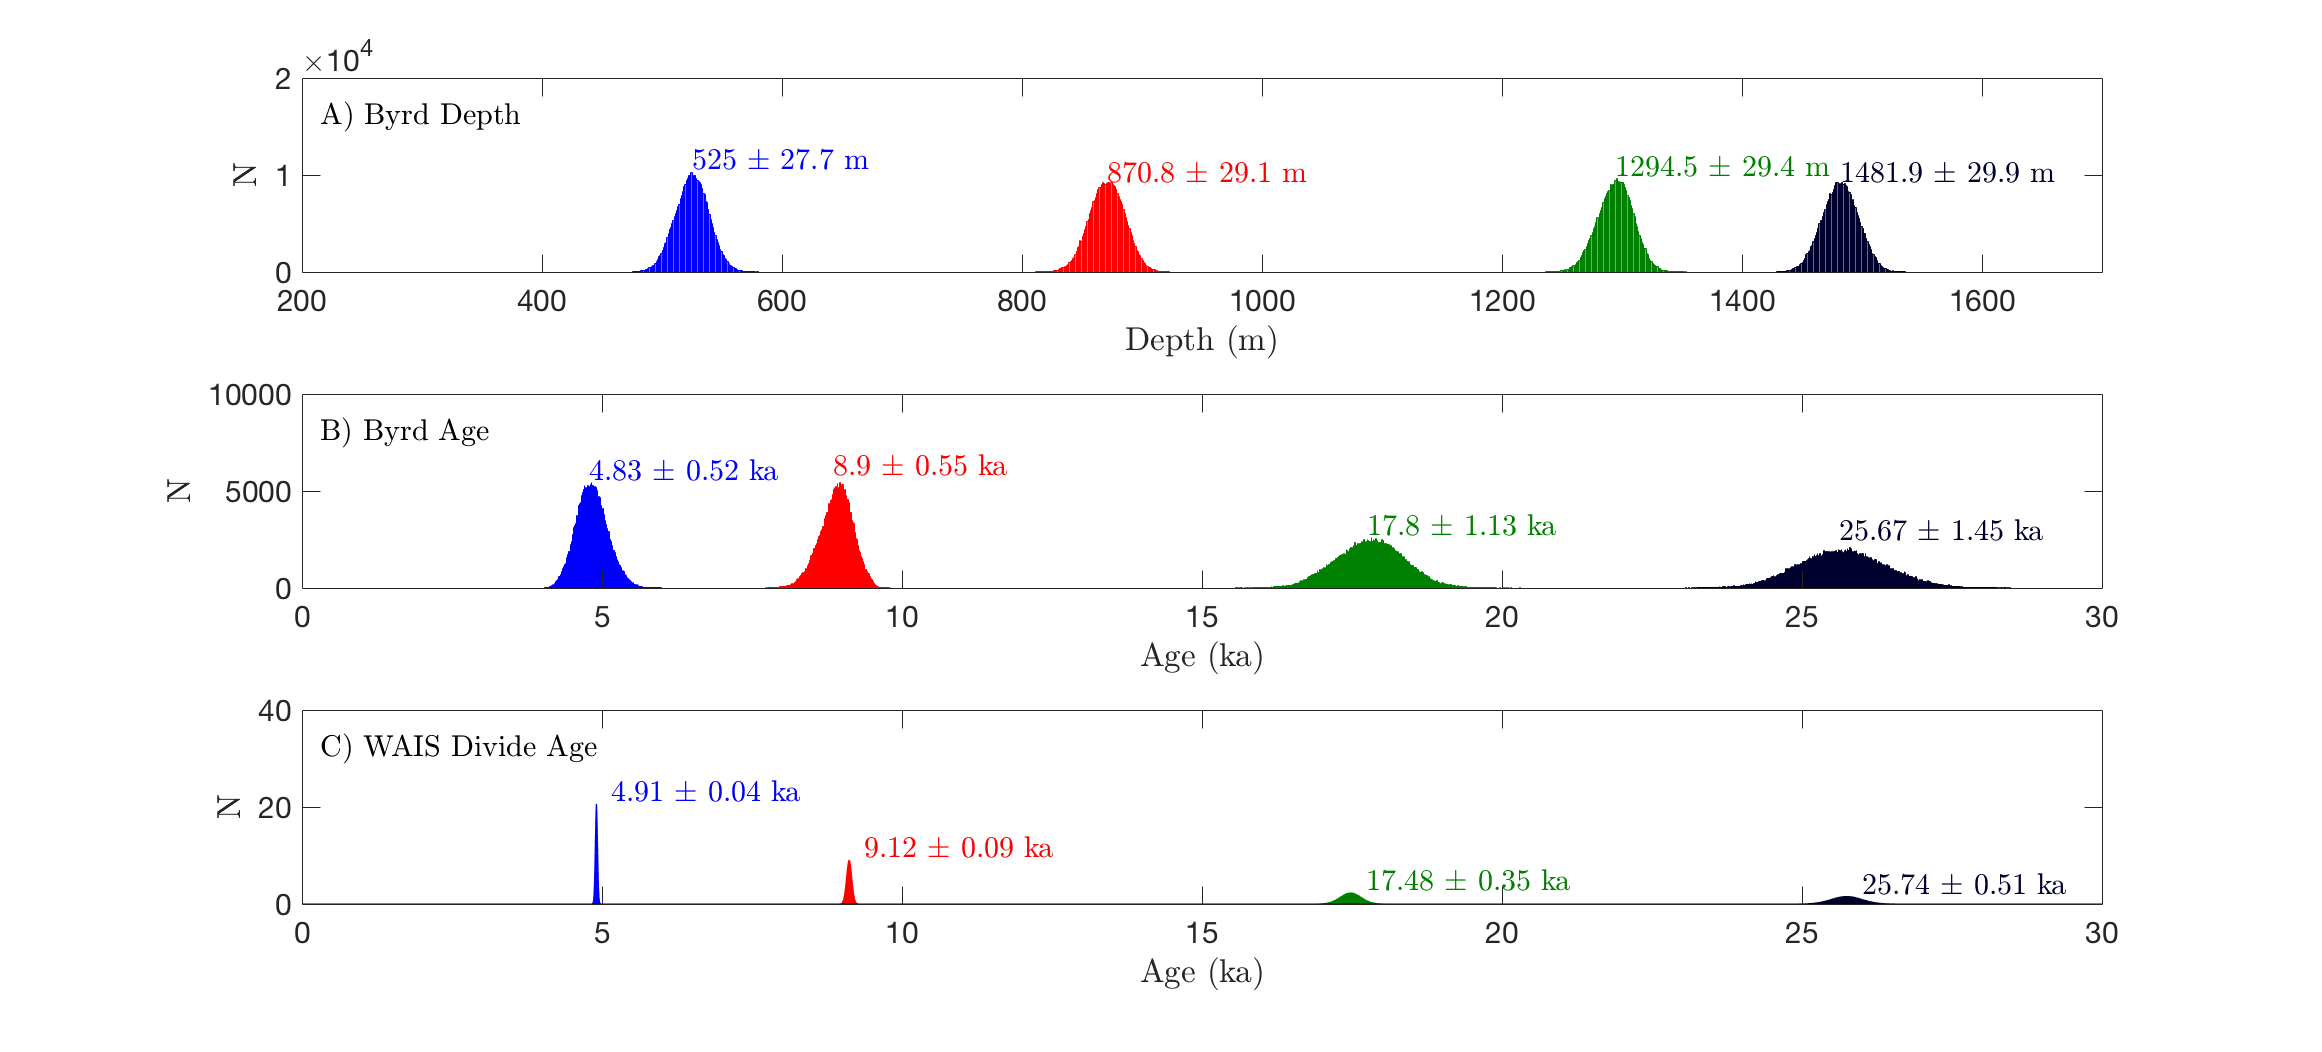
\includegraphics[scale=0.4]{/Users/gail/Documents/Research/Projects/age-depth-firninvert/analysis/figures/agedepthhisto}
}
%\captionsetup{width=.9\textwidth}
\caption{Posterior probability distributions of depth (top) and age (bottom) of 4 radar reflectors at the Byrd ice core. The width of the age and depth histograms for the Byrd ice core chronology represent uncertainty estimated by the methods used here.}
\label{fig:layer_histo}
\end{figure*}

\begin{figure*}[h]
%\begin{center}
\centering
\makebox[\textwidth][c]{\includegraphics[scale=0.6]{/Users/gail/Documents/Research/Projects/age-depth-firninvert/analysis/figures/spaghetti}}
%\captionsetup{width=.9\textwidth}
\caption{Modeled age-depth relationship with uncertainty compared to measured volcanic chronology from \citet[]{hammer1997} (open circles). The WAIS Divide ice core chronology \citep{buizert2015} as a black line. Blue triangles show the age-depth of 4 radar reflectors at each of the Byrd and WAIS Divide ice cores; these reflectors are assumed isochronous and so expected to be the same age at either ice core.}
%\end{center}
\label{fig:spaghetti}
\end{figure*}

\subsection{Error budget}
To evaluate how much errors in each parameter contribute to uncertainties in age and depth of radar reflectors, we consider how uncertainty in reflector age and depth change when each parameter is assumed to be known with no error. To do so, we hold each model parameter fixed at its optimal value (Figure~\ref{fig:layer_histo}). If there is no change in the distribution of reflector age and depth, error in that model parameter has no influence on the result.

%To evaluate which parameters contribute most to uncertainties in the age and depth of radar reflectors, we compute an error budget based on the sensitivity of the estimated age and depth of each reflector to the value of each estimated parameter. %By fixing the estimated depth to each reflector. 
We find errors in depth contribute 25\%, 37\%, 77\%, and 43\% to uncertainty in depth to reflectors 1, 2, 3, and 4, respectively. This suggests that deeper in the ice column an increasing portion of uncertainty in age is from errors in reflector depth. However, high reflector SNR (and therefore radar range precision) can mitigate this effect. As seen in Figure~\ref{fig:layer_histo}, the deepest observed reflector, which may be expected to have the largest depth uncertainty, instead has relatively high SNR and therefore low uncertainty.

Uncertainty in age is also sensitive to the accumulation rate profile which accounts for up to 40\% of the age uncertainty of each reflector. 
Accumulation rates in localized portions of the ice column do not individually influence the age uncertainty as much as the full accumulation rate profile, but rates in the upper part of the ice column have more impact due to their influence on the age of ice below. Other individual ice flow parameters play a far smaller role in the error budget.



% In doing so, we find the error due to radar range precision, $\epsilon_{prec}$, is the most significant contributor to uncertainty in reflector depth. Further, we find estimates of accumulation rate, $\dot{a}$, contribute up to 20\% of the uncertainty in reflector age. Other parameters, including $\dot{a}$ for individual depths in the ice column, have either small or ambiguous contributions to the overall uncertainty in age and/or depth. Such ambiguities may be the result of potentially complex correlation between parameters. 


% \subsection{Parameter correlations}\label{sec:ke}
%\counterwithin{figure}{section} %reset figure numbering
% The ability to explore parameter correlations is one advantage of our method. We expect there to be correlation between parameters in this study due to stratigraphic dependence of age and depth in the ice column. 

%% However, we find no notable correlation between most parameters. Exceptions include correlation between the depth of radar reflectors and $d_{firn}$ (Figure~\ref{fig:depthCorrelation}) and between accumulation rates in the bottom half of the ice column and the ratio of surface to basal ice velocity, $q$ (Figure~\ref{fig:accumCorrelation}). Even in these limited cases, correlations are generally low.



%Figure \ref{fig:depthCorrelation} shows radar depth estimates are positively correlated. This follows from the dependence of relative reflector depth based on stratigraphy; if the uppermost reflector is deeper in the ice column, all other reflectors must also be relatively deeper as well.

%% show little correlation to each other, while they are more strongly correlated with the firn correction, $d_{firn}$. This follows from the fact that changes in $d_{firn}$ will directly shift the depth of each radar reflector. On the other hand, accumulation rate estimates in the bottom half of the ice column are correlated both to each other and to the ice flow parameter, $q$. This coincides with increasing uncertainty in the accumulation rate prior to the LGM (Figure~\ref{fig:accumdepth}), likely because of difficulty estimating the transition between the LGM accumulation rate minimum and earlier accumulation rates (below 1850 m) where we lack volcanic age constraints. This may indicate priors on accumulation rate depth are of particular importance where there is a lack of other constraining data and that our result could be improved with more informative accumulation rate priors in this region of the ice column.

%%that our priors play an important role in estimating the value of accumulation rate and therefore the result could be improved with a more informative prior. This is particularly true at the bottom of the ice column, where neither volcanic chronology data nor radar data is available to constrain the accumulation rate.



%%We see correlation between some accumulation rate parameters (left side of Figure~\ref{fig:accumconvergence}). This may indicate we could have combined these accumulation rate depth bins. Figure~\ref{fig:accumCorrelation} shows a correlation matrix between pairs of accumulation rate parameters. Along the diagonal are histograms of each accumulation rate parameter. Pairs of accumulation rate parameters to not tend to be very correlated and only one pair of accumulation rate parameters has $R^2 > 0.5$. In general, $R^2$ values are highest between accumulation rates in the lower part of the ice column, where parameter values are more difficult to constrain due to a lack of data and flatter age-depth profile.



%%Figure~\ref{fig:flowparamconvergence} shows the results of inverting for several model parameters in this problem, including flow parameters such as $q$ as well as ice property parameters such as $v_{ice}$. The results show the parameters are not correlated with one another and do seem to convergence to most-likely solutions.

%%As expected, estimates of the depth of the four radar reflectors at each iteration are correlated to each other because knowledge of the depth and age of each layer informs the relative depth and age of all other reflectors. The resulting accumulation rate profile is shown in Figure~\ref{fig:accumdepth}. The accumulation rate profiles more closely resemble a climatic record, for which the accumulation rate was lower during the Last Glacial Maximum% ($\sim$ 1400 m depth)
% . 

% \begin{figure*}[ht]
% %\begin{center}
% \centering
% \makebox[\textwidth][c]{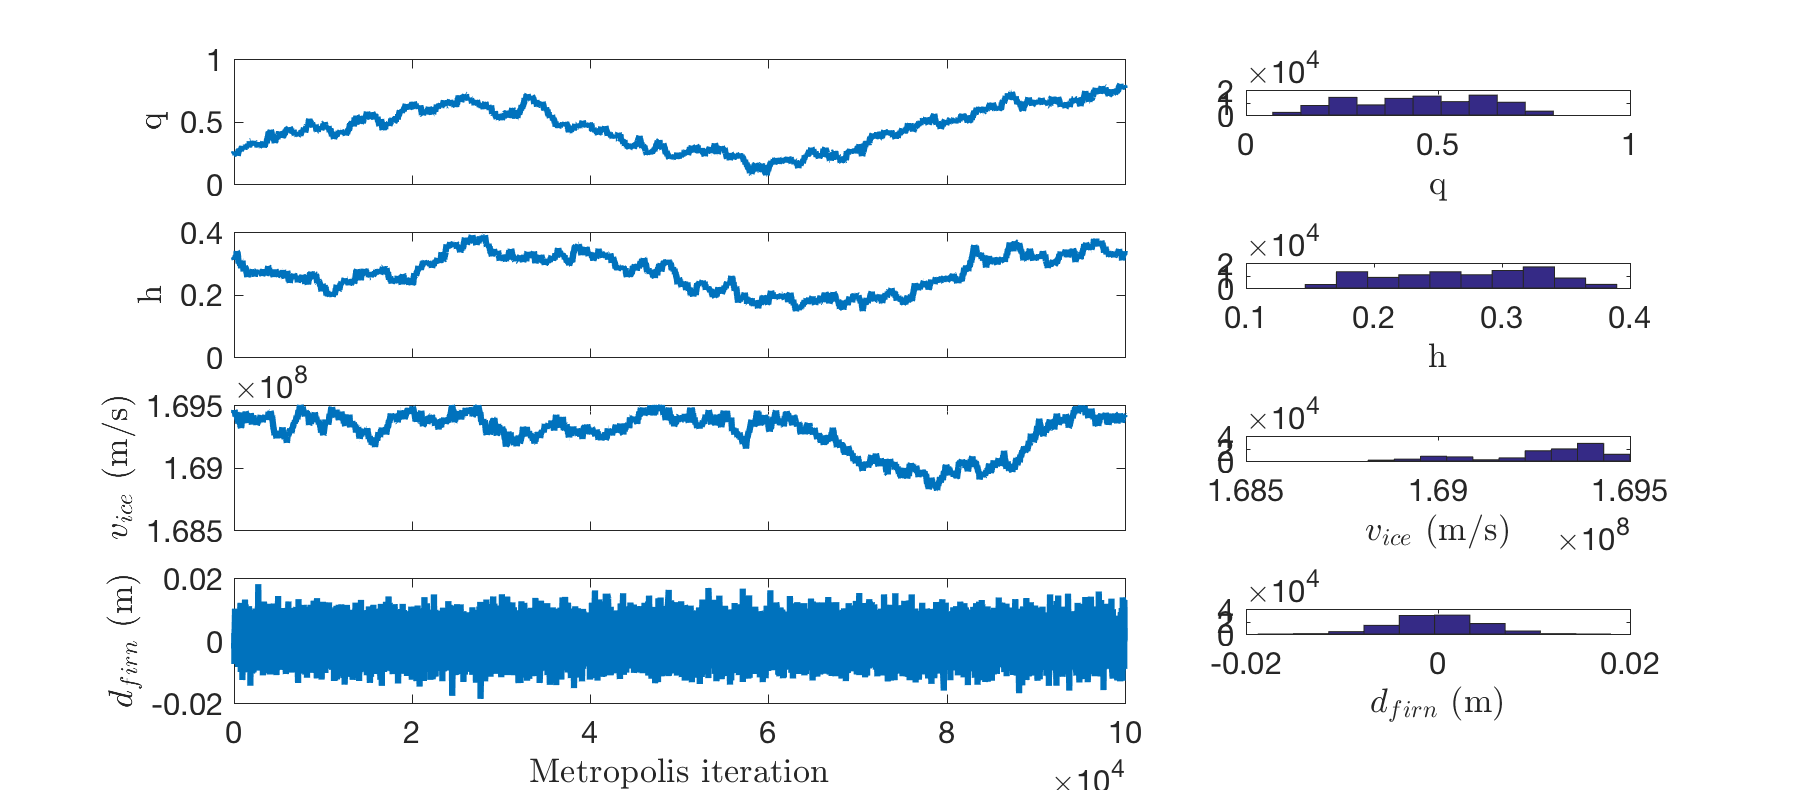
\includegraphics[scale=0.4]{../analysis/figures/convergence1}}
% %\captionsetup{width=.9\textwidth}
% \caption[]{Left: Flow parameter values at each accepted Metropolis iteration for parameters $q$ (top), $h$, $v_{ice}$, and $d_{firn}$ (bottom). The parameter values do not appear correlated. Right: Histograms of the parameter values shown in the left column. Histograms show the parameter values converging.}
% %\end{center}
% \label{fig:flowparamconvergence}
% \end{figure*}

%Accumulation rate is divided into 10 parameters, each covering a depth bin of $\sim$200 m. This allows for variation in the accumulation rate over time, as expected. The resulting accumulation rate profiles are shown in Figure~\ref{fig:accumdepth}. As discussed elsewhere in the Supplemental Information, these profiles have been regularized to preferentially select those which do not exhibit unrealistic variability. In Figure~\ref{fig:accumdepth}, they have been additionally sorted by cost to demonstrate the relative quality of the accepted solutions.

\begin{figure*}[ht]
%\begin{center}
\centering
\makebox[\textwidth][c]{\includegraphics[scale=0.3]{/Users/gail/Documents/Research/Projects/age-depth-firninvert/analysis/figures/accumdepthSorted}}
%\captionsetup{width=.9\textwidth}
\caption{Accumulation rate as a function of ice depth colored by cost value which reflects each solution's fit to data. (Accumulation rate functions associated with lower cost are expected to be better solutions.) Accumulation rate is estimated in 10 depth bins at $\sim$200 m depth intervals. Transitions between these intervals have been smoothed in this figure for ease of viewing.}
%\end{center}
\label{fig:accumdepth}
\end{figure*}

%To further explore the accumulation rate solutions, we look at the accepted parameter values and their convergence over all iterations. As seen in the right side of Figure~\ref{fig:accumconvergence}, the accumulation rate solutions do not converge as readily as other parameters, leaving wider distributions exhibiting more uncertainty in our estimates of accumulation rate. This may mean that our priors play an important role in estimating the value of accumulation rate and therefore the result could be improved with a more informative prior. This is particularly true at the bottom of the ice column, where neither volcanic chronology data nor radar data is available to constrain the accumulation rate.


\begin{figure*}[ht]
%\begin{center}
\centering
\makebox[\textwidth][c]{
\includegraphics[scale=0.5]{/Users/gail/Documents/Research/Projects/age-depth-firninvert/analysis/figures/paramHist}}
%\captionsetup{width=.9\textwidth}
\caption{Posterior probability distributions of inverted parameters, including accumulation rate, $q$, $h$, $v_{ice}$, $\epsilon_{firn}$, and $S$. Accumulation rate paramter values are assigned to 200 m depth intervals indicated by the subscript. While a few parameter distributions appear non-gaussian, parameter values are well sampled and generally single-peaked. The precision parameter, $S$, has an expected gamma distribution and $\epsilon_{firn}$ is normally distributed, as expected.  }
%\end{center}
\label{fig:paramhist}
\end{figure*}



% \begin{figure*}[ht]
% %\begin{center}
% \centering
% \makebox[\textwidth][c]{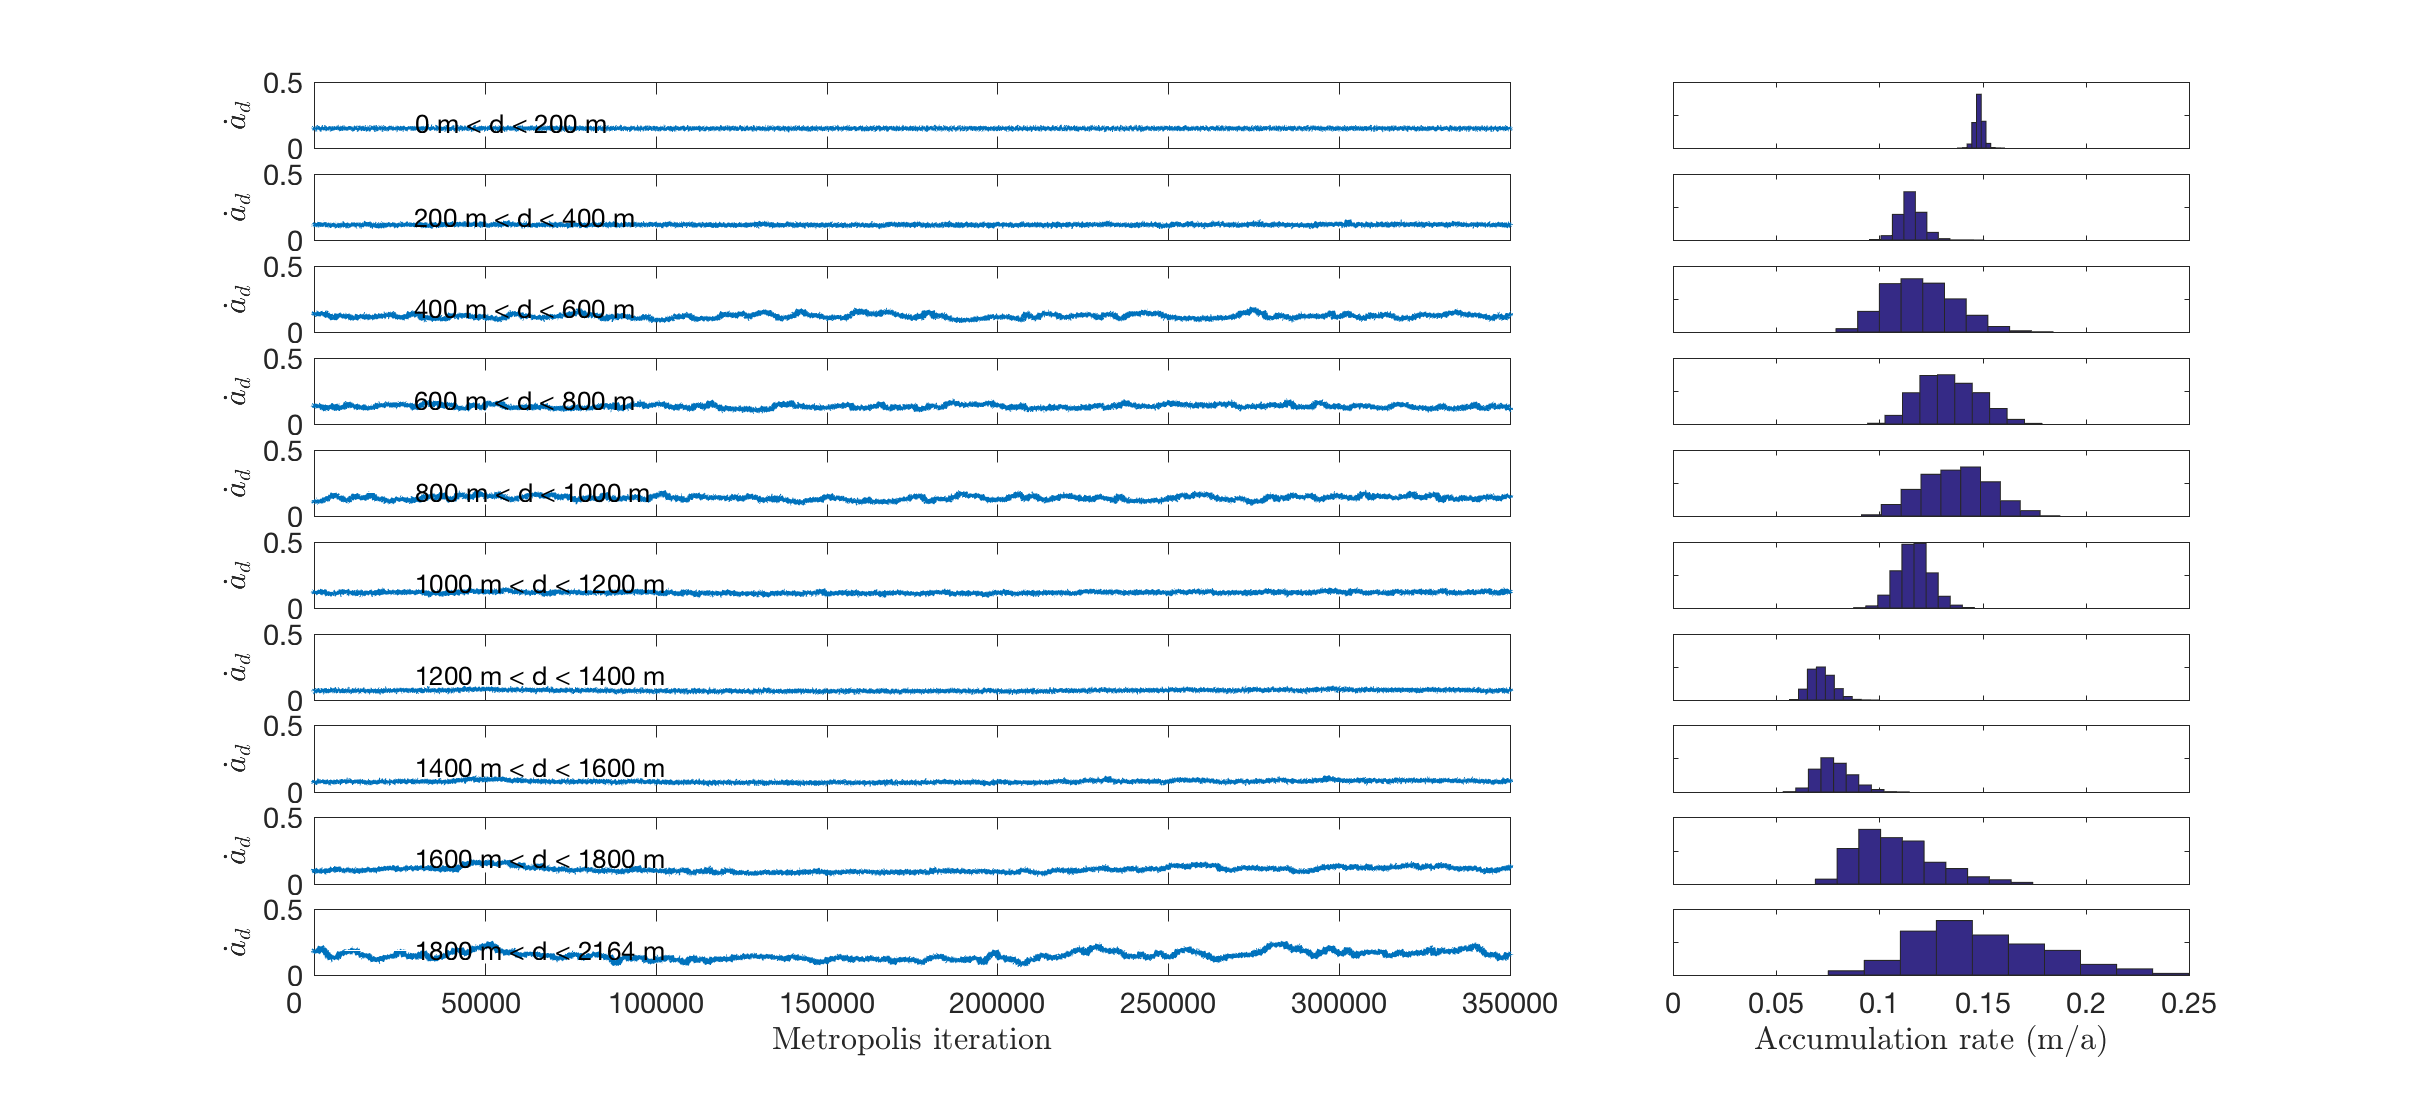
\includegraphics[scale=0.4]{../analysis/figures/convergence2}}
% %\captionsetup{width=.9\textwidth}
% \caption[]{Left: Values of each accumulate rate parameter (in each of 10 depth bins, shallowest at top). Right: Histograms of the parameter values at left. Certain depth bins appear to be correlated and the histograms of values are wider, indicating the accumulation rate parameters are slower to converge and more uncertain.}
% %\end{center}
% \label{fig:accumconvergence}
% \end{figure*}

% \begin{figure*}[ht]
% %\begin{center}
% \centering
% \makebox[\textwidth][c]{\includegraphics[scale=0.5]{../../age-depth-firninvert/analysis/figures/depthCorrelation}}
% %\captionsetup{width=.9\textwidth}
% \caption[]{Correlation between depth estimates and firn correction, $d_{firn}$.}
% %\end{center}
% \label{fig:depthCorrelation}
% \end{figure*}

% \begin{figure*}[ht]
% %\begin{center}
% \centering
% \makebox[\textwidth][c]{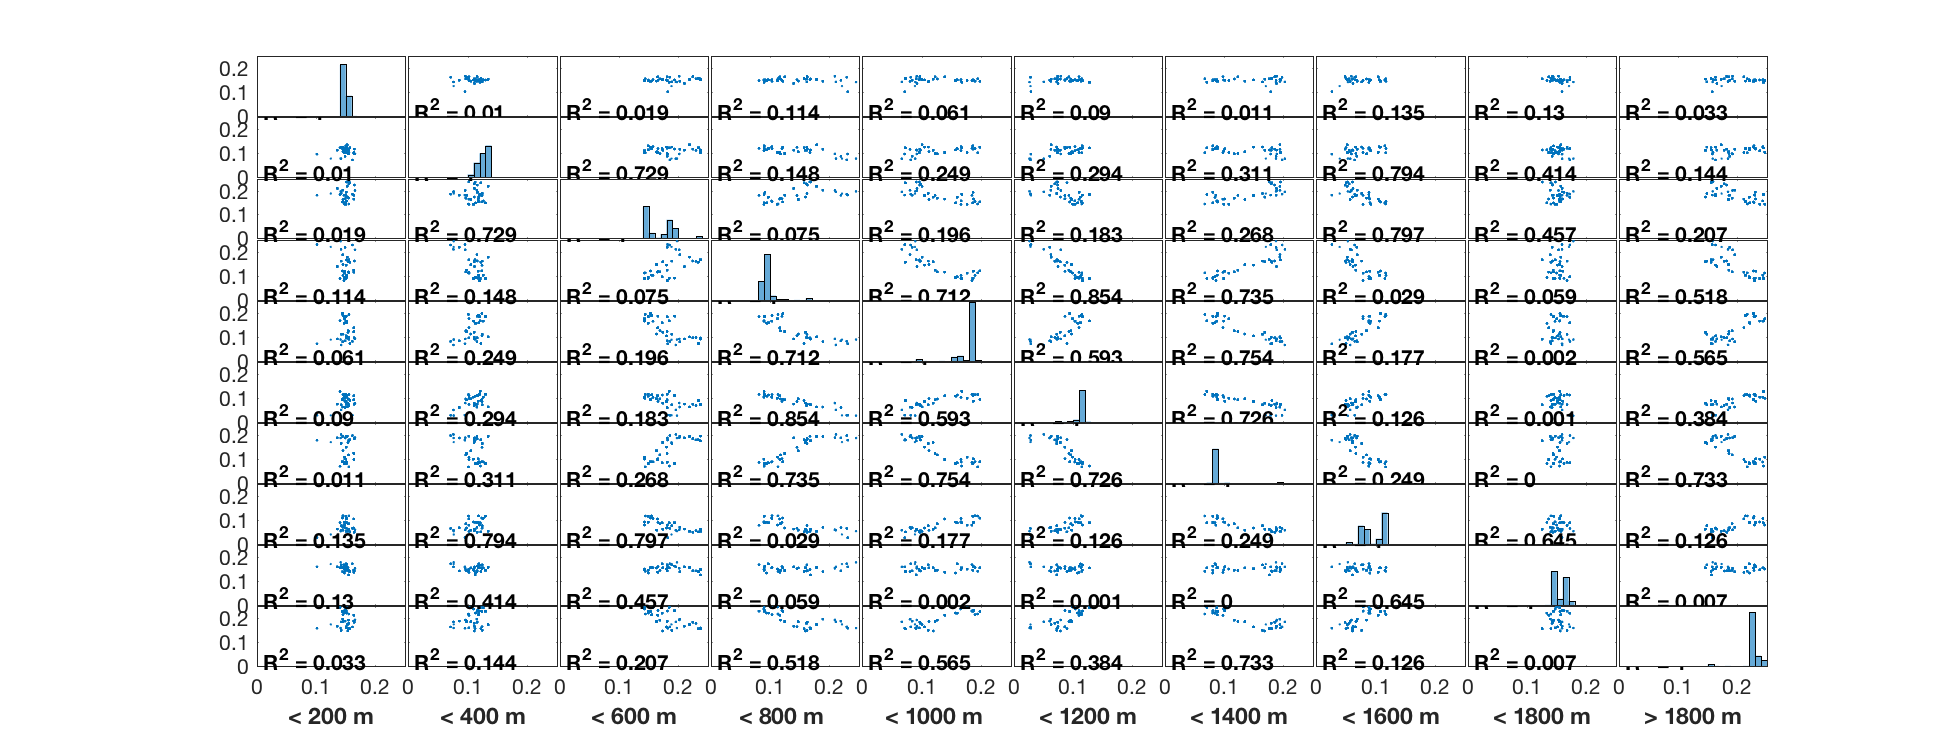
\includegraphics[scale=0.4]{/Users/gail/Documents/Research/Projects/age-depth-firninvert/analysis/figures/accumCorrelation.png}}
% %\captionsetup{width=.9\textwidth}
% \caption{Correlation of 4 deepest accumulation rate bins with the ratio of surface to bed ice velocity, $q$.}
% %\end{center}
% \label{fig:accumCorrelation}
% \end{figure*}




 